\begin{figure}[h!]
    \centering
    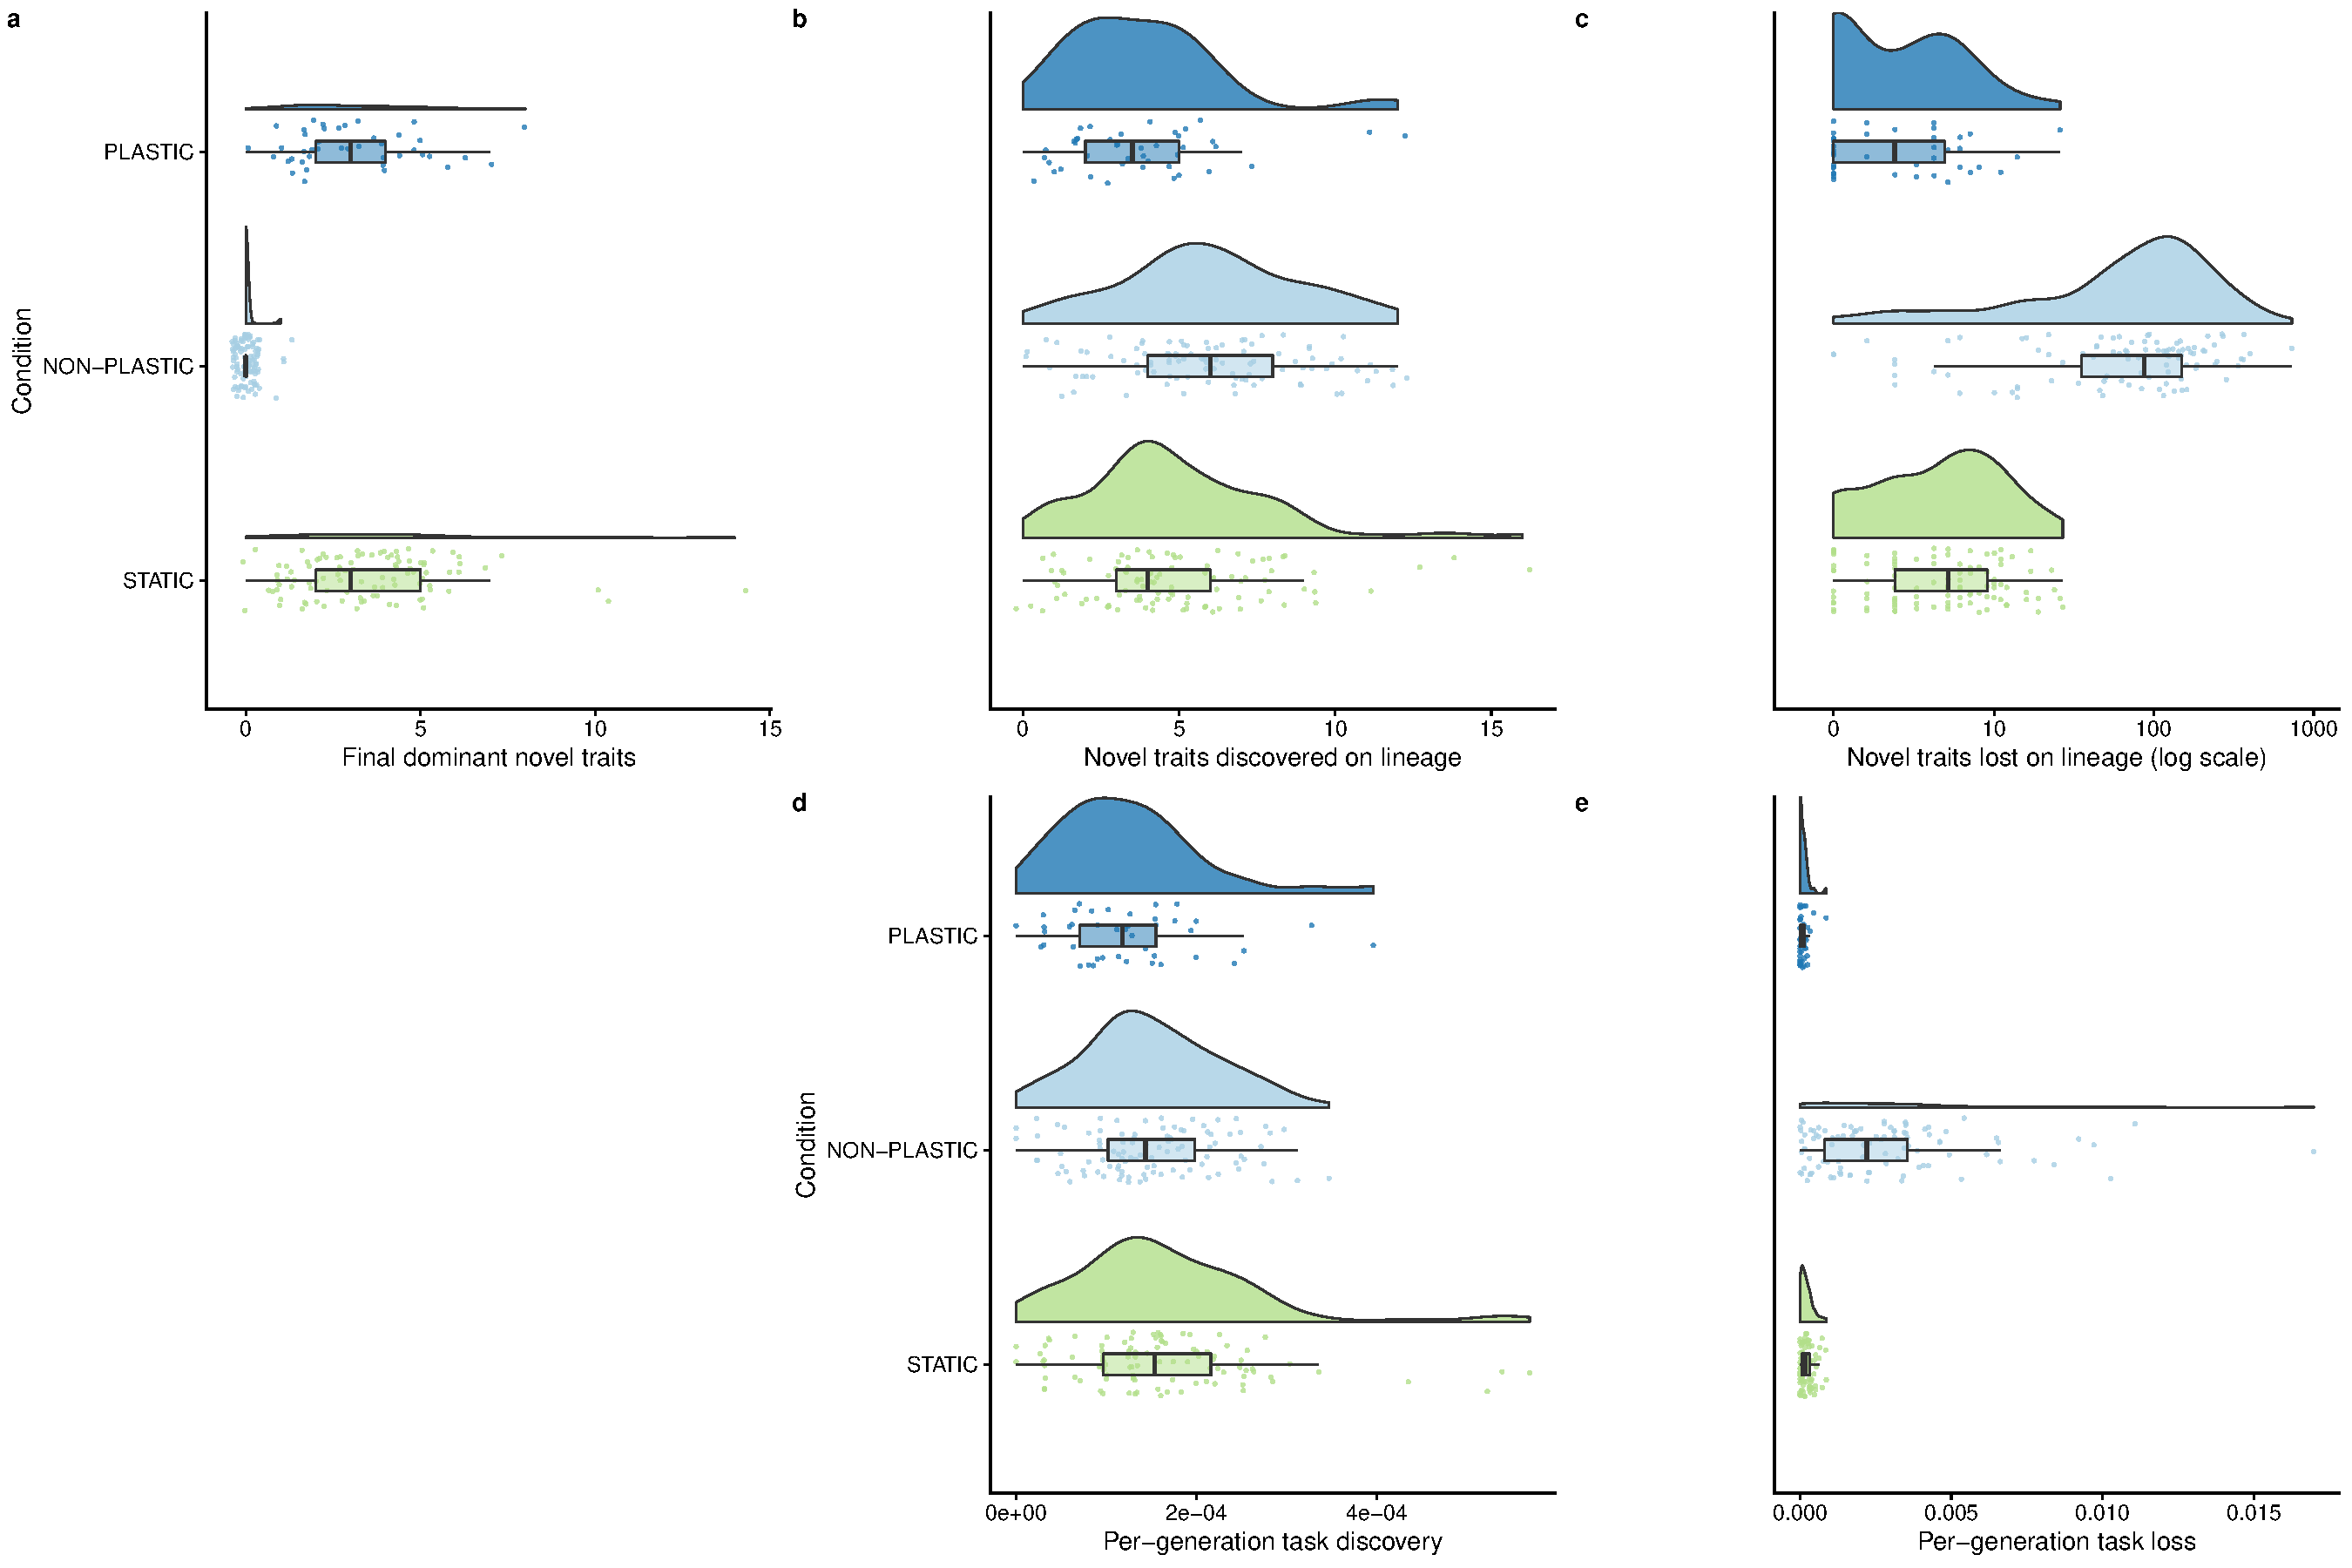
\includegraphics[width=0.9\textwidth]{media/complex-traits-panel.pdf}
    \caption{\small
    \textbf{Novel task evolution.}
    Raincloud plots of 
    (a) final novel task count,
    (b) novel task discovery,
    (c) novel task loss,
    (d) novel task discovery frequency,
    and (e) novel task loss frequency.
    See Table \ref{tab:metrics-definitions} for descriptions of each metric.
    Each plot is annotated with statistically significant comparisons (Bonferroni-corrected pairwise Wilcoxon rank-sum tests).
    Note that adaptive phenotypic plasticity evolved in \novelTraitsPlasticReps\ of \novelTraitsReplicates\ replicates from the PLASTIC treatment during phase one of Experiment II; we used this more limited group to seed the resulting \novelTraitsPlasticReps\ phase-two PLASTIC replicates.
    }
    \label{fig:complex-traits}
\end{figure}